\chapter{Stereoscopic Visualization}

InVesalius supports stereoscopic visualization of 3D models. First a surface (see chapter~\ref{cap_surface}) or an active volumetric visualization (see chapter~\ref{cap:vis_vol}) must be created. Then, click the icon (shown in Figure~\ref{fig:ster}) on the bottom right part of the interface and choose the desired projection type (Figure~\ref{fig:st_menu}).


\begin{figure}[!htb]
\centering

\includegraphics[scale=0.6]{3D_glasses.png}
\caption{Shortcut to activate stereoscopic viewing methods.}
\label{fig:ster}
\end{figure}

\begin{figure}[!htb]
\centering
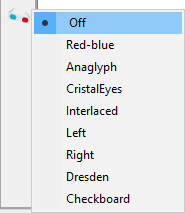
\includegraphics[scale=0.4]{st_menu_en.png}
\caption{Different methods of stereoscopic visualization.}
\label{fig:st_menu}
\end{figure}

InVesalius supports the following types of stereoscopic viewing:

\begin{itemize}
	\item Red-blue
	\item Anaglyph
	\item CristalEyes
	\item Interlaced
	\item Left
	\item Right
	\item Dresden
	\item Checkboard
\end{itemize}

Figure~\ref{fig:st_surf_methods} presents three different types of projections.


\begin{figure}[!htb]
  \centering
  \subfloat[Interlaced]{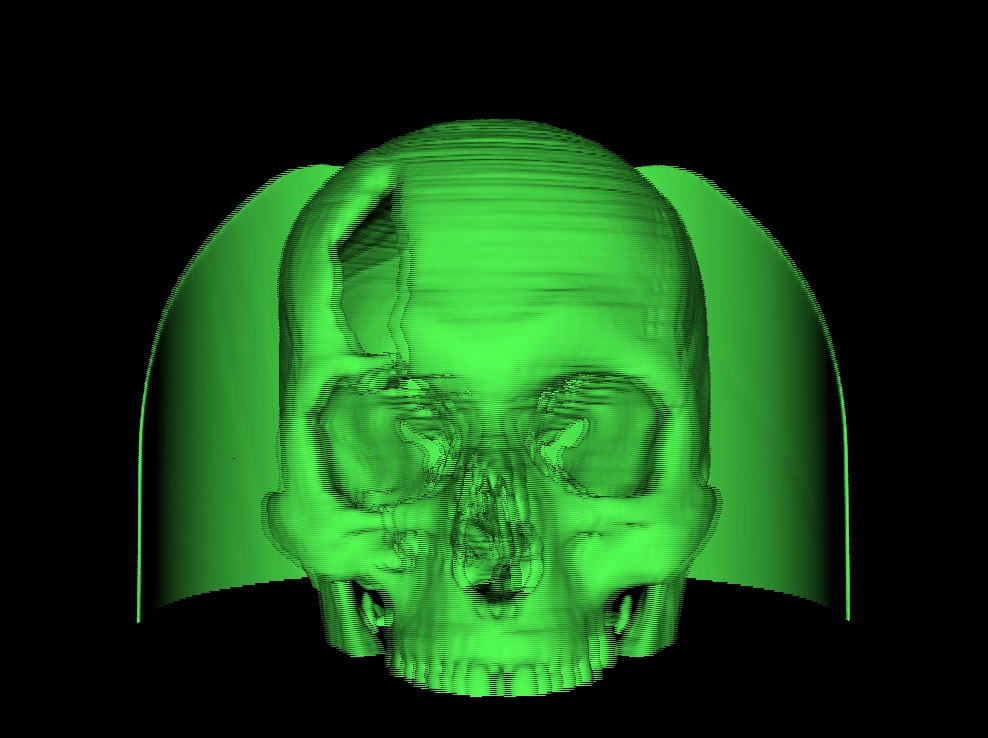
\includegraphics[width=0.3\textwidth]{st_surf_interlaced.jpg}} \qquad
  \subfloat[Anaglyph]{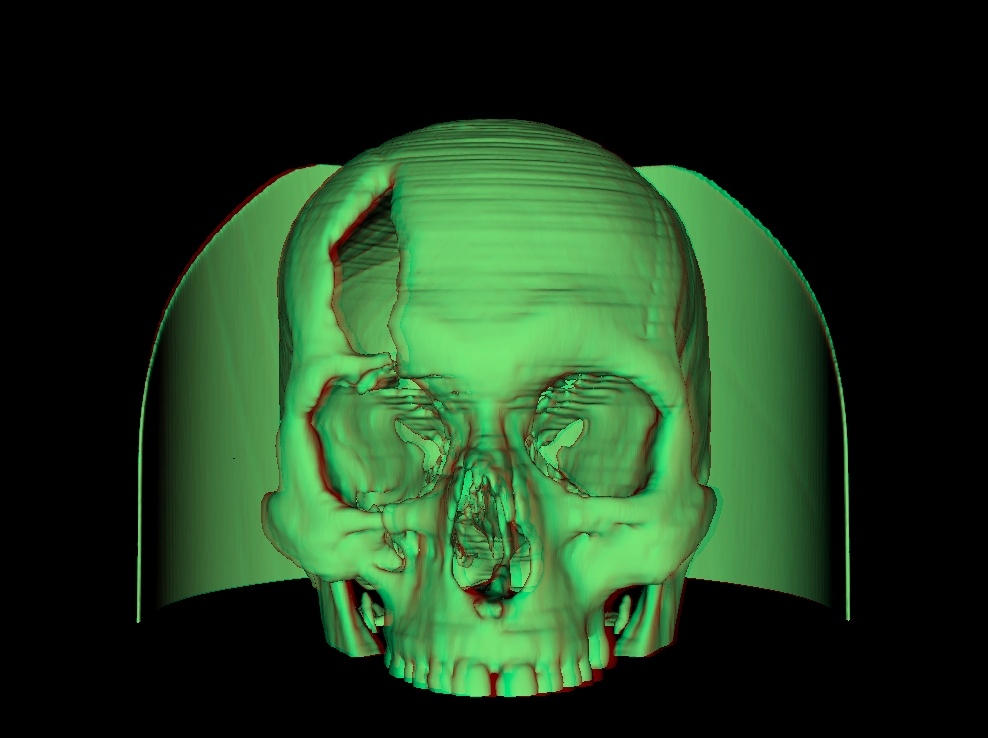
\includegraphics[width=0.3\textwidth]{st_surf_anaglyph.jpg}} \qquad
  \subfloat[Red-blue]{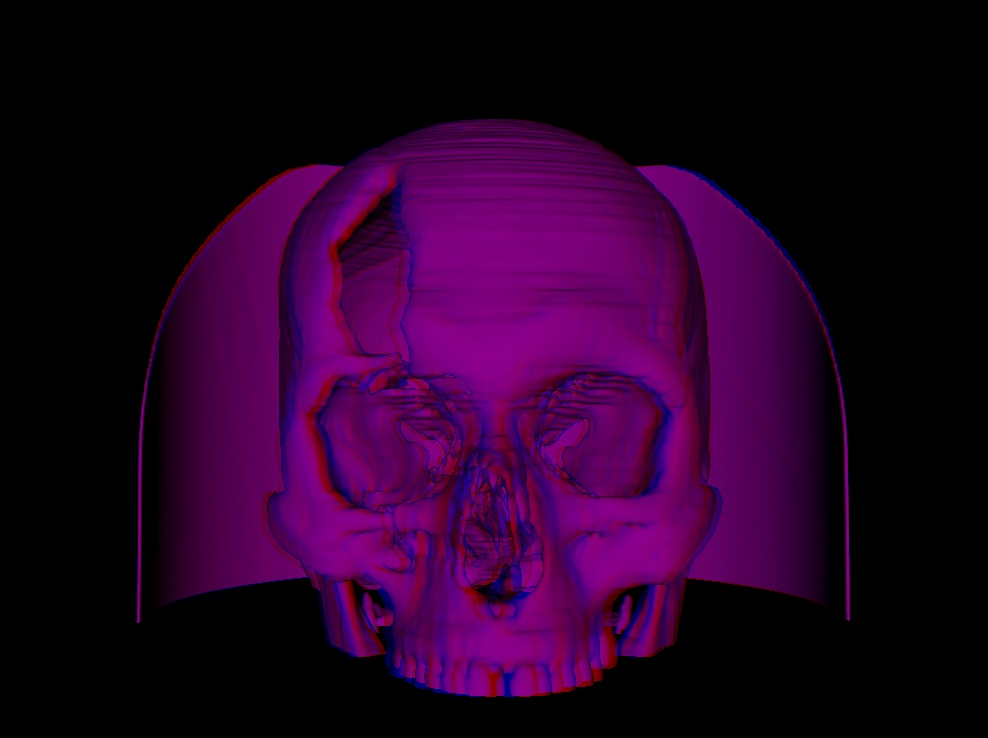
\includegraphics[width=0.3\textwidth]{st_surf_red_blue.jpg}}  
  \hfill
  \caption{Example of different methods of stereoscopic applied on a surface.}
  \label{fig:st_surf_methods}
\end{figure}